\documentclass[a4paper,11pt]{article}
\usepackage[utf8]{inputenc}
\usepackage{amsmath}
\usepackage{amsfonts}
\usepackage{amssymb}
\usepackage{graphicx}
\usepackage[font=scriptsize]{caption}
\usepackage[font=scriptsize]{subcaption}
\usepackage{wrapfig}
\usepackage[backend=biber]{biblatex}

\addbibresource{nn.bib}
\renewcommand\thesubsection{\alph{subsection}}


%opening
\title{One-dimensional traveling waves in neural columns}
\author{Vince Baker, advisor: Dr. Luis Cruz Cruz\\ Drexel University Department of Physics}

\begin{document}

\maketitle

\begin{abstract}
Cortical traveling waves have been observed in vivo and in simulations of recurrent networks.
These traveling waves explain various features of cortical dynamics including spike timing variability and correlated fluctuations in membrane potential.
In this work we examine the firing dynamics of neural column structures similar to those found in the cortex.
We find that traveling waves are evoked by random background stimulus in networks with distance-dependent connectivity and propagation delay.
We determine that the propagation velocity of the waves is determined by both the action potential propagation time and the topology of the column.
This topological dependence of wave propagation may indicate a functional role of the cortex organization into columns.

\end{abstract}

\section{Introduction} 
Traveling waves of cortical neuron activation have been observed in vivo, in vitro and in silico. 
Proposed functions of these traveling waves include motor coordination, place field coordination in the hippocampus, and spatiotemporal processing in the visual cortex \cite{muller2018}. 
Advanced experimental techniques that achieve the required spatial and temporal resolution \cite{shoham1999} to capture the mesoscopic traveling waves have focused on lateral activity near the cortical surface, and simulations of traveling waves in a 2-D sheet of neurons have been performed \cite{keane2015}. 
\\
Several types of cortical propagating waves have been studied.
Slow, large-scale wave activity have been observed in sleep and anesthetized states \cite{muller2018}.
Advances in optical imaging techniques using voltage-sensitive dye provided sufficient spatial resolution to observe local area mesoscopic traveling waves in the awake cortex \cite{wu2008}.
Stimulus-evoked mesoscopic waves have been observed in the mammalian visual and auditory cortex \cite{reimer2010}\cite{muller2018}.
Experimental observation of mesoscopic traveling waves in the cortex has largely focused on lateral waves within the layers \cite{muller2018} as vertical penetration is more difficult to image. 
\\
In this work we explore the dynamics of traveling waves along neural structures with one long dimension, similar to column structures that may be found in the cortex.
We find that these traveling waves in one dimension can propagate in simulated neural column structures with certain properties including distance-dependent connectivity and a mix of excitatory and inhibitory neurons. 
We observe wave properties including creation from background stimulus, annihilation between waves, and a wave velocity that is determined by both the action potential propagation speed and the column topology. 

\section{Methods}
We simulated the dynamics of a small neural column to explore neuron synchronization.
Our network geometry is based on the model presented in \cite{markram1998}.
An example neural column composed of 135 neurons on a unit grid spacing, 3x3 neurons wide and 15 neurons high as shown in figure \ref{fig:column_structure}.
\begin{figure}[!htb]
 \caption{Example column structure used in this research, $\lambda=2.5$,$C=1$. The left image shows the connections between neurons in the column, the color scale indicates connection length. The right image shows inter-neuron connectivity for excitatory connections (green) and inhibitoruy connections (red).}
 \label{fig:column_structure}
 \centering
   \includegraphics[width=\textwidth]{fig/lambda2}
\end{figure}
The neurons are connected with a strong local connectivity according to the distance-based connection probability:
\begin{align}\label{eq:connectivity}
 P_{a,b} &= C \times e^{-(D(a,b)/\lambda)^2}
\end{align}
Where $D(a,b)$ is the distance between neuron A and B and $\lambda$ and $C$ are parameters of the connection model.
\\ \\
We model the neurons using the Izhikevich model \cite{izhikevich2003} to allow us to explore the neural dynamics.
The Izhikevich model uses two coupled differential equations with two variables and four parameters:
\begin{align}
 v^\prime &= 0.04v^2+5v+140-u+I \label{eq:neuron_v} \\
 u^\prime &= a(bv-u)\\
 \text{if } &v>30: v\leftarrow c, u\leftarrow u+d
\end{align}
This is a simplified model of a two-dimensional dynamical system.
This model has been used to reproduce common neural firing patterns.
There is MATLAB code available \cite{izzy_code} that implements this neural model with fixed, single-time-step action potential propagation.
The model parameters for excitatory and inhibitory neurons are shown in Table \ref{tab:izzy_params}.
We define $\mathcal{U}\{a,b \}$ as a uniform random variable drawn on $[ a,b ] $.
\begin{table}[!h]
 \caption{Izhekevich model parameters}
 \label{tab:izzy_params}
 \centering
 \begin{tabular}{l|c|r}
  \textbf{Parameter} & \textbf{Excitatory} & \textbf{Inhibitory} \\
  \hline
  a & 0.02 & 0.02+$\mathcal{U}$(0,0.08) \\
  b & 0.2 & 0.25-$\mathcal{U}(0,0.05)$\\
  c & -65+$\mathcal{U}(0,10)^2$ & -65 \\
  d & 8-$\mathcal{U}(0,6)$& 2 \\
 \end{tabular}
\end{table}
\\
In the Izhikevich model when a neuron fires the action potential propagates to the target neuron at the next time step.
The action potential from the firing neuron is added to the target neuron current $I$ (Eq \ref{eq:neuron_v}).
We enhanced the available MATLAB code for the Izhikevich model to incorporate a more realistic propagation model while still minimizing computational complexity.
Our model incorporates a propagation delay $\tau_{ij}=\kappa D(i,j)$ porportional to the inter-neuron distance $D(i,j)$ between neurons $i$ and $j$. 
The parameter $\kappa$ ranges from 0 (action potentials propagate to the target neuron in the next time step) to 4. 
We also model an exponentially decaying synapse respone $I(t)=e^{-(\frac{t}{\sigma_s})^2}$ with a time constant of $\sigma_s=4~ms$.
\\ \\
The connection strengths between neurons is based on the original Izhikevich work.
The strength for connections from presynaptic neuron $i$ to postsynaptic neuron $j$ depends on whether $i$ is inhibitory or excitatory.
\begin{align}
 S_{ij}^{excitatory} &= K \times \mathcal{U}\{0,\frac{1}{2} \} \\
 S_{ij}^{inhibitory} &= K \times \mathcal{U}\{-1,0 \} 
\end{align}
The parameter K is used to adjust the overall connection strength: $K=1$ corresponds to the original model in \cite{izzy_code}. \\
The current in Equation \ref{eq:neuron_v} includes all incoming stimulus from other neurons.
With our models for action potential propagation and synapse response, the total current to neuron $i$ can be written:
\begin{align}
 I_i(t) &= \sum_{j\ne i} \sum_{t^\prime_j} S_{ij}  \delta(t-t^\prime_j-\tau_{ij})e^{-(\frac{t-t^\prime_j-\tau_{ij}}{\sigma_s})^2}
\end{align}
Where the $t^\prime_j$ are all firing times of neuron $j$ and $\delta$ is the Kronecker delta.
\\ \\
The current in Equation \ref{eq:neuron_v} also includes any stimulus applied as part of the experiment.
We perform experiments using both a uniform background stimulus and a step stimulus.
Our model for uniform background stimulus to a neuron $i$ depends on whether $i$ is inhibitory or excitatory, following Izhikevich's original model.
The uniform background stimulus is:
\begin{align}
 I_i^{excitatory} &= M \times \mathcal{U}\{0,1 \} \\
 I_i^{inhibitory} &= \frac{2}{5} M \times \mathcal{U}\{0,1 \}
\end{align}
The parameter $M$ is used to adjust the overal strength of the stimulus, $M=1$ corresponds to the original model in \cite{izzy_code}.
\\
A step stimulus is used when measuring the speed of a traveling wave.
The step stimulus is applied uniformaly to neurons in the lowest 5 layers of the column.
The stimulus starts at $t=20~ms$ and lasts for $20~ms$ during which the affected neurons receive a constant current input of strength 5.
This generates a single traveling wave with a determined start time, simplifying the propagation velocity measurement.
\\ \\
We capture the firing events from all neurons in each simulation.
We then perform a spatial clustering operation to identify spatiotemporal regions with a high firing density.
This clustering operation removes random background firing activity.
We then identify and label the traveling wave structures that evolve over time as shown in Figure \ref{fig:wave_analysis}.
\begin{figure}[!htb]
 \centering
 \begin{subfigure}{0.33\textwidth}
  \centering
  \includegraphics[width=\textwidth]{fig/2x2_firings}
 \end{subfigure}%
 \begin{subfigure}{0.33\textwidth}
  \centering
  \includegraphics[width=\textwidth]{fig/2x2_density_filter}
 \end{subfigure}%
 \begin{subfigure}{0.33\textwidth}
  \centering
  \includegraphics[width=\textwidth]{fig/2x2_wave_IDs}
 \end{subfigure}%
 \caption{Wave processing. The raw firing events (left) are filtered in time and position (center) to remove background firing events. The individual waves are then labeled with unique numbers (right, wave numer shown as color scale).}
 \label{fig:wave_analysis}
\end{figure}
\\
Several useful measurements can be extracted from the labeled wave data, including the wave start positions and wave propagation speed.
We define the ``wave firing fraction`` as the fraction of the neuron firing events (Figure \ref{fig:wave_analysis}, left) that are associated with the labeled traveling waves.
\\ \\
Simulations are run with a $0.5~ms$ time step except where noted.
The traveling wave behavior looks qualitatively similar at time steps from $1~ms$ down to $10~\mu s$ (Figure \ref{fig:time_step}).
\begin{figure}[!htb]
 \centering
 \includegraphics[width=\textwidth]{fig/TimeStepEffect}
  \caption{A traveling wave experiment at 4 different time scales. The qualitative behavior is the same.}
 \label{fig:time_step}
\end{figure}


\section{Results}
We determine the conditions for traveling waves to propagate in our simulated neural columns.
We first examine the connectivity between the neurons and find traveling waves for columns with local connectivity.
We then examine the impact of actional potential propagation delay, finding that traveling waves are supported in fully-connected columns when the propagation delay is porportional to distance.
We find that the excitatory/inhibitory balance plays a role in traveling wave propagation and determines the character of column activity.
Finaly, we show that the traveling wave propagation speed depends on both the action potential propagation speed as well as the column topology. \\
The baseline model for all experiments are a column of 2x2x100 neurons where $80\%$ of the neurons are excitatory except where noted.
Connectivity parameters are $\lambda=2.5$ and $C=1$.
The exponential synapse response time $\sigma_s$ is always $4~ms$.
The Izhekevich model parameters are as described in Methods, with conenction strenght parameter $K=5$ and stimulus strength parameter $M=5$ except where noted.

\subsection{Connectivity}
We first investigate the impact of connectivity on traveling wave formation.
We varied the connection strength parameter $K$ and observed the conditions under which uniform background stimulus would produce traveling waves.
In Figure \ref{fig:strength_effect} we show typical traveling waves for three different values of $K$.
\begin{figure}[!htb]
 \caption{Effect of connection strength on traveling wave formation. $K$ is the connection strength parameter. At $K=2$ the firing events appear random, while at $K=6$ traveling waves are clearly evident.}
 \centering
   \includegraphics[width=0.75\textwidth]{fig/ConnectionStrengthWaves}  
 \label{fig:strength_effect}
\end{figure}
\\
At low connection strength $K=2$ the firing events appear random.
Traveling waves are evident at a higher connection strength of $K=4$.
We see visually that the traveling wave patterns dominate the firing activity at $K=6$. \\
We performed 50 simulations values of $K$ from $2$ to $6$ at intervals of $0.5$ and determine the wave firing fraction as decribed in methods (Figure \ref{fig:conn_fraction}).
Below $K=3.5$ no traveling waves are detected.
We observe the transition at $K=3.5$ where traveling waves are observed but most of the firing events are still random.
From $K=3.5$ to $K=5$ the wave firing fraction is porportional to $K$, indicating that traveling waves become more dominant as the neurons become more strongly connected.
At $K>5$ more than $90\%$ of the firing events are part of a traveling wave.
\begin{figure}[!htb]
 \caption{Traveling waves emerge at $K=3.5$. As the connection strength increases the traveling waves dominate all firing events in the column.}
 \centering
   \includegraphics[width=0.5\textwidth]{fig/ConnectionStrengthWaveFraction}  
 \label{fig:conn_fraction}
\end{figure}
\\
We also observe in Figure \ref{fig:strength_effect} that traveling waves annihilate each other when they meet.
The annihilation effects can be explained by the refractory period of the neurons.
Neurons that are activated by one traveling wave will be hyperpolarized and less likely to fire if another traveling waves arrives within a short time period.

\subsection{Delay}
To investigate the impact of delay we simulate a column with complete connectivity corresponing to $\lambda \rightarrow \infty$: all neurons are connected with probability 1 to all other neurons.
This is analagous to the original Izhikevich simulation \cite{izzy_code} that demonstrated synchronized firing in a completely connected neural field with random background stimulus.
We first simulated the column with a fixed action potential propagation delay of $1~ms$ regardless of inter-neuron distance.
The result was highly synchronized simultaneous firing among all neurons in the column (Figure \ref{fig:sync_fire}). \\ 
We then incorporated our distance-dependent action potential propagation with the $\kappa$ parameter set to 1.
The firing is still highly synchronized, but traveling waves are now evident (Figure \ref{fig:sync_fire_delay}).
This demonstrates that one dimensional traveling waves can emerge from fully-connected networks if the propagation time is porportional to the inter-neuron distance.
\begin{figure}[!htb]
  \centering
  \begin{minipage}{0.45\textwidth}
      \centering
      \includegraphics[width=0.95\textwidth]{fig/IzzySync}
      \caption{Synchronized, simultaneous firing in a completely connected column with constant propagation delay.}
      \label{fig:sync_fire}
  \end{minipage}\hfill
  \begin{minipage}{0.45\textwidth}
      \centering
      \includegraphics[width=0.9\textwidth]{fig/IzzySync_Delay}
      \caption{Traveling waves emerge when the propagation delay is porportional to the inter-neuron distance. }
      \label{fig:sync_fire_delay}
  \end{minipage}
\end{figure}
Previous work (\cite{ermentrout2001}, Figure 1) classifies several architectures for apparent traveling waves in the cortex.
One architecture, ''Delayed Excitations from a Single Oscillator``, is a periodic source driving a sequence of excitable neurons with increasing time delays, but no connectivity between the neurons.


\subsection{Excitatory/Inhibitory Balance}
The excitatory/inhibitory balance is known to have a significant impact on neural network dynamics \cite{keane2015}. 
In our model we do not observe traveling waves if less than $40\%$ of the neurons are excitatory.
As the fraction of excitatory neurons increase we observe traveling wave patterns emerge from the background firing events.
As the excitatory fraction increases more of the firing events occur within waves structures (Figure \ref{fig:excitatory_effect}).
When all neurons are excitatory the traveling waves are the dominat mode of firing, with substantially all of the firing events contained within traveling waves. \\
\begin{figure}[!htb]
 \caption{Excitatory/inhibitory balance effect on traveling waves.. 
	  For columns with $<40\%$ excitatory neurons no waves are observed.
	  As the excitatory fraction approaches 1 nearly all firing events are part of traveling waves.
	  Error bars are 1 $\sigma$, 100 trials per measurement.
	  }
 \label{fig:excitatory_effect}
 \centering
   \includegraphics[width=0.5\textwidth]{fig/ExcitatoryWaves}
\end{figure}

\subsection{Propagation speed}
To examine the velocity of the traveling waves we performed 50 velocity for measurements for two parameters of interest.
We varied the propagation delay constant $\kappa$ from (1 to 4) and the cross section of the column (2x2, 2x3, 3x3).
The results are shown in Figure \ref{fig:delay_topology}.
\begin{figure}[!htb]
 \caption{Wave speed is inversely porportional to $\kappa$ as expected. Wave speed also increases with the column cross-section.Mean values with $1\sigma$ errorbars, 50 trials.}
 \label{fig:delay_topology}
 \centering
   \includegraphics[width=0.75\textwidth]{fig/WaveSpeed_DelayTopology}
\end{figure}
\\
We see that both the delay constant and the column topology influence the propagation speed.
Increasing the inter-neuron actiona potential delay slows the traveling wave propagation.
Waves travel faster in columns with larger cross-sections. 

\subsection{Wave Initiation}
It appears that columns have preferential wave initiation sites.
Figure \ref{fig:wave_initiation} shows all the wave initiation sites for 100 simulations of a column.
It is clear that traveling waves are more likely to begin at certain regions in the column.
\begin{figure}[!htb]
 \caption{Wave initiation sites, 100 trials with randomized exciation. Initation events are shown in the left figure. A histogram of initiation positions for all waves is shown on the right.}
 \label{fig:wave_initiation}
 \centering
   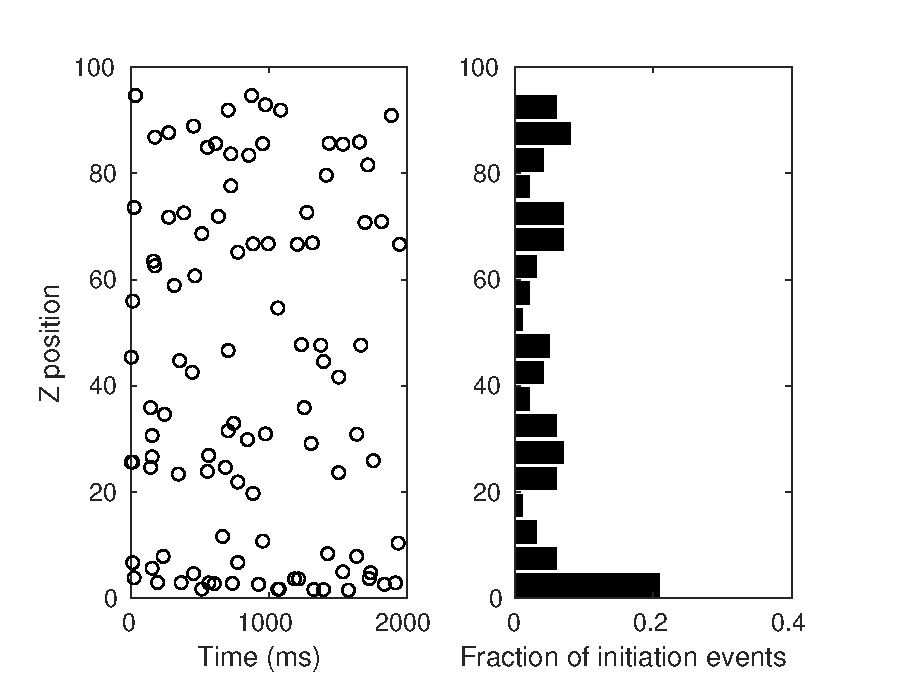
\includegraphics[width=0.75\textwidth]{fig/InitiationSites_100sims}
\end{figure}
We are currently unable to explain the preferential initiation sites in term of connectivity or excitatory/inhibitory balance. 
\\
We also observed that, when generating traveling waves from a step stimulus that certain sections of the column showed a higher density of firing activity.
An example measurement of the firing density is shown in Figure \ref{fig:wave_density}.
\begin{figure}[!htb]
 \caption{Density of firing events in a traveling wave initiated from a step stimulus. The traveling wave is shown on the left, a histogram of firing events by position is shown on the right.}
 \label{fig:wave_density}
 \centering
   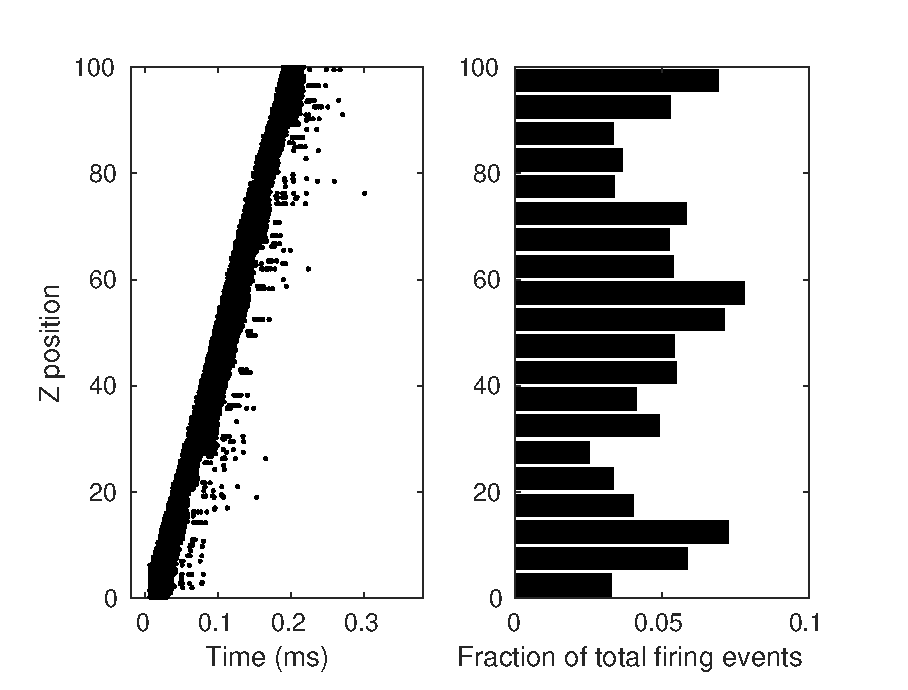
\includegraphics[width=0.75\textwidth]{fig/ImpulseWaveDensity}
\end{figure}
While examining the preferntial wave initiation sites emerging from random stimulus we discovered a correlation to the firing density observed in the same columns under step simulus.
The wave initiation sites and wave density of the same column are shown in figure \ref{fig:initiation_density}.
\begin{figure}[!htb]
 \caption{Wave initiation (left) and wave density (right) for the same column.}
 \label{fig:initiation_density}
 \centering
   \includegraphics[width=0.75\textwidth]{fig/InitiationCorrelationHistogram}
\end{figure}
There appears to be an anticorrelation between wave density under a step stimulus and the likelihood of wave initiation under a uniform background stmiulus.
To test this hypothesis we create 100 columns, applied both background stimulus and step stimulus, and measured the correlation between wave inititation and wave density at the positions of the column (Figure \ref{fig:initiation_density_corr}).
Although there is substantial variation between columns we measure a consistently negative correlation coefficient (mean -0.18, std 0.20).
\begin{figure}[!htb]
 \caption{Correlation between wave initiation and wave density.}
 \label{fig:initiation_density_corr}
 \centering
   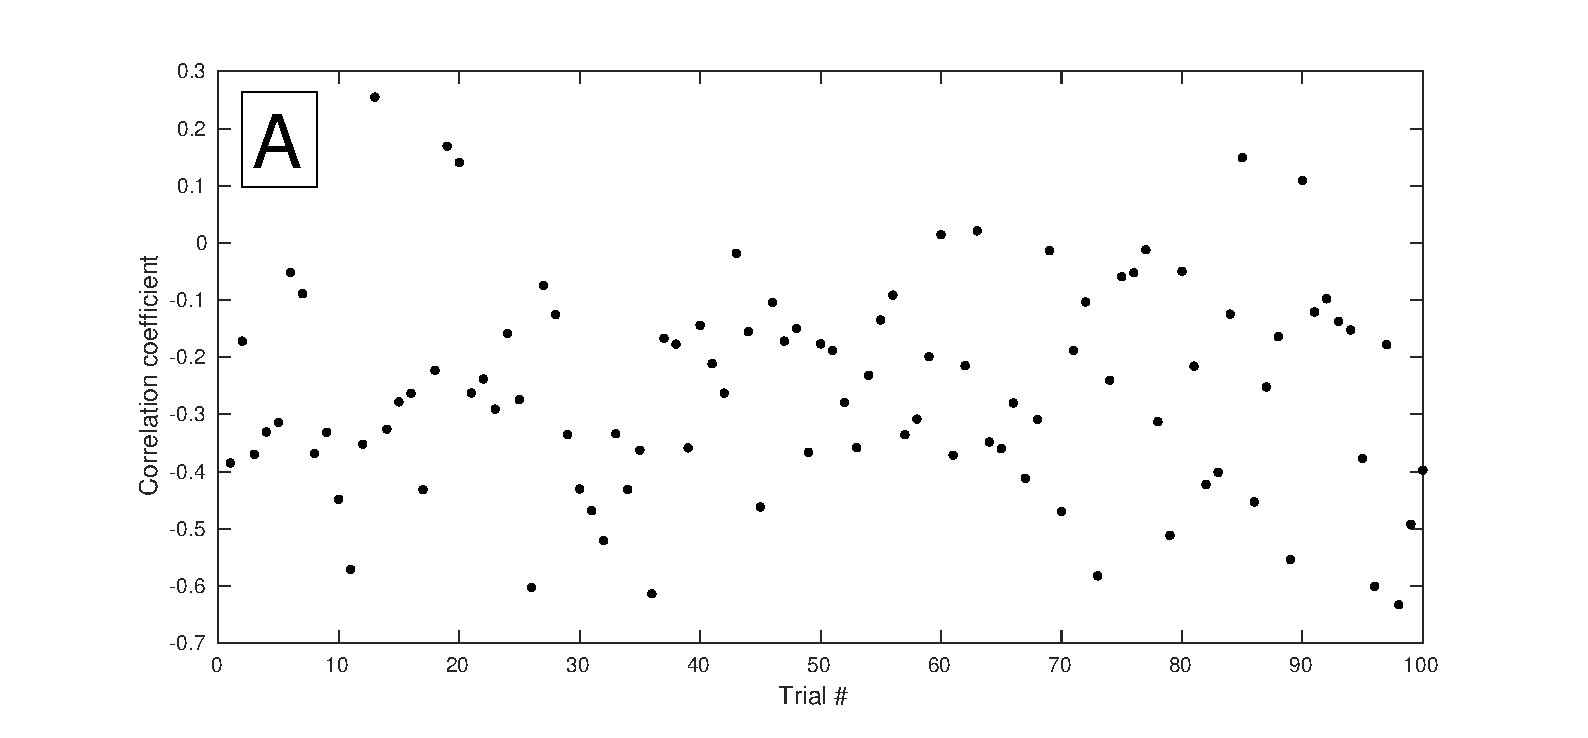
\includegraphics[width=0.75\textwidth]{fig/InitiationCorrelation}
\end{figure}

\subsection{Column ensembles}
We simulate an ensemble of four columns. 
The individual columns are 2x2x50, with $80\%$ excitatory neurons, connection strength $K=5$, connection model parameters $\lambda=2.5$ and $C=1$.
All neurons in all columns were stimulated with a background stimulus, strength $K=5$.
The spacing between the columns was varied from 2 to 10. 
At an inter-column spacing of 2 the ensemble is a single column with a 4x4 cross section.
At an inter-column spacing of 10 there were no connections between the neurons in the columns.
Ensembles with intermediate inter-column spacings have some degree of connectivity between the columns.
\begin{figure}[!htb]
 \caption{Increasing inter-column distance reduces the connectivity between columns (top row). The firing events (bottom row) are color-coded by column number. }
 \label{fig:ensemble}
 \centering
   \includegraphics[width=\textwidth]{fig/ColumnEnsemble}
\end{figure}
\\
With inter-column spacing of 2 the ensemble fires as a single column.
As the spacing increases to 5 the connectivity between columns becomes weaker than the intra-column connectivity.
There is still correlation between the traveling waves in the four columns.
As the spacing increases further there is no connectivity between the columns.
The traveling waves in the columns are now uncorrelated.

\section{Discussion}
We have demonstrated that representative column structures can support traveling waves.
Various parameters determine traveling wave formation and propagation including the connectivity, connection strength, excitatory/inhibitory balance and action potential propagation delay.
Columns with local connectivity support traveling waves, consistent with other simulations and experimental studies of cortical traveling waves.
We have also shown that even a fully-connected column exhibits traveling waves if the action potential propagation time depends on the inter-neuron distance. 
\\
Traveling waves in neurons have previously been analyzed as a set of coupled local oscillators.
Although the Izhikevich model is capable of producing self-resonant oscillations when tuned appropriately, the model parameters used in this work did not show any evidence of self-oscillation.
The waves studied in the present work seem to fall instead into the general category of propagating pulses in an excitable network described in \cite{ermentrout2001}. 
\\
In \cite{muller2018} the authors noted that mesoscopic traveling waves typically have propagation speeds from 0.1 to 0.8 meters per second, consistent with axonal conduction speed of unmyelinated fibers.
Our linear model of synpatic conduction delay is linear with inter-neuron distance, with a porportionality constant $\kappa$.
We expected longer synaptic conduction delays to result in slower wave propagation.
The column topology can also influence the propagation speed.
Columns with a larger cross-section have a larger number of neurons and synapses for a given length, providing more pathways for the traveling wave to propagate.
The propagation delay parameter $\kappa$ does effect the wave propagation as expected, but the effect is not linear.
If the traveling wave velocity was determined by the action potential propagation speed we would expect to see wave velocity of 1000 units/second with $\kappa=1$.
Instead the wave velocity is less than half the simple prediction (Figure \ref{fig:delay_topology}).
A four-fold increase in $\kappa$ does not reduce the traveling wave propagation speed by a factor of 4. 
\\
The column topology also has a significant impact on wave propagation speed, with waves in the thinner 2x2 columns traveling about $25\%$ slower than in the 3x3 column.
Real columns will have a less regular structure and we may expect them to show a more continuous variation in wave propagation speed. 
The variations in propagation speed could be an important feature of traveling waves in organizing cortical activity.
\\
Ensembles of coupled columns showed various degrees of correlation in trave wave activity. 
The inter-column coupling, combined with the distribution of wave parameters among the individual columns, suggest a possible computational role for column organization.
Columns may carry information between cortical layers in the form of traveling waves. 
Naturally occuring differences in wave propagation will result in phase differences between waves in different columns.
Ensembles of columns might perform nonlinear filtering functions through the interaction of the traveling waves within the individual columns.


\clearpage
\printbibliography

\end{document}
